% !TeX document-id = {55cdd1f2-c708-43a6-9dcf-ca7bc9e91f17}
% !BIB program = biber
\documentclass[10pt]{beamer}

\usetheme{scilifelab}
\usepackage{appendixnumberbeamer}

\usepackage{booktabs}
\usepackage[scale=2]{ccicons}

\usepackage{hyperref}
\hypersetup{colorlinks=true, linkcolor=scAqua, urlcolor=scAqua, citecolor=scAqua}
%\usepackage{natbib}

\usepackage{pgfplots}
\usepgfplotslibrary{dateplot}

\usepackage{xspace}
\newcommand{\themename}{\textbf{\textsc{scilifelab}}\xspace}
\newcommand{\credit}[1]{{\par \raggedleft \scriptsize \mdseries \color{mDarkBrown} #1 \par}}
\newcommand{\citeme}[1]{{\xspace\color{scAqua} \scriptsize \cite{#1}}}

\title{Token(s) of love}
\subtitle{Potentials and pitfalls of LLM use in our daily work tasks}
\date{February 14, 2025}
\author{Matthias Zepper, PhD}
\institute{NGI Stockholm, Genomic Focus Meeting}
\titlegraphic{\hfill
\includegraphics[height=1cm]{./additional_graphics/SciLifeLab_Logotype_Green_POS.png}}

\begin{document}

\maketitle

\begin{frame}{Valentine's day 2025: Mankind in love with generative AI models}
\begin{figure}
	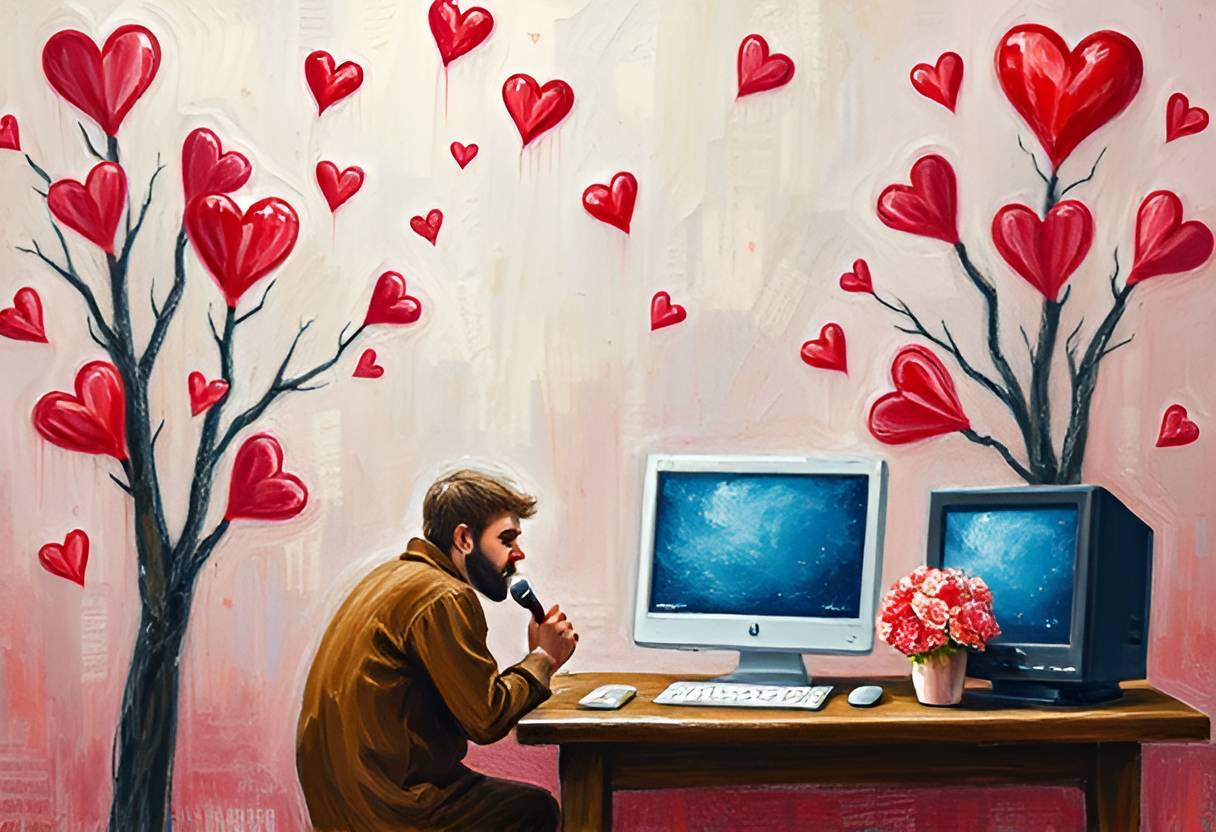
\includegraphics[width=0.8\textwidth]{figures/Valentine_s_Day_oil_painting_mathematic_matrices_formulas_and_computers}
	\caption{A person in love with AI models and computers. Created with the open-weights 'FLUX.1 [schnell]' model by Black Forest Labs.}
\end{figure}
\credit{https://blackforestlabs.ai, https://github.com/black-forest-labs/flux}
\end{frame}


\begin{frame}{Encounters with AI generated content are inevitable...*}
	
	Of course, I can help write your meeting invitation email!
	Dear colleagues,
	You are hereby invited to the next Focus Meeting on Friday, February 14th at 9:00 AM in Gamma-2-Earth-G2593. I’m sorry, but as an AI Language Model, I cannot participate in meetings.
	Embark on a deep dive of the AI landscape and delve into the intricate world of Large Language Models (LLMs).
	Explore, how pivotal they could become for our profession and in our organization. Based on the information provided we’ll begin with the fundamentals of LLMs, cover some major applications and lastly address their suitability for real-world use cases at the NGI.
	Looking forward to a lively exchange of ideas
	Best,
	[Your Name]
	
	\credit{*actually not AI generated, because it turns out ChatGPT is a poor impersonator of its earlier versions}
\end{frame}
% % % % % % % % % % % % % % % % % % % % % % %55


 

% % % % % % % % % % % % % % % % % % % % % % % % %





\begin{frame}[standout]{aasdas}
UAG
\end{frame}


\begin{frame}{Encounters with AI generated content are inevitable...}
	\begin{figure}
		\hspace*{-1cm} 
		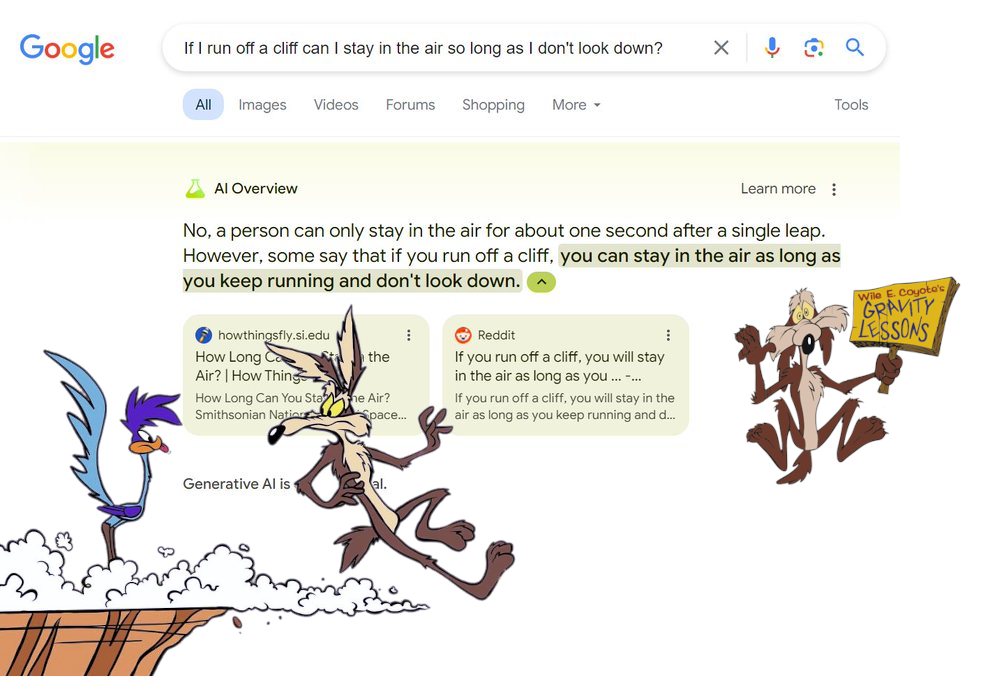
\includegraphics[height=0.97\textheight]{figures/Cliffs.png}
	\end{figure}
\end{frame}

% % % % % % % % % % % % % % % % % %

\begin{frame}{Twisted transcription}
\begin{columns}[T,onlytextwidth]
	\column{0.5\textwidth}
	
	\begin{alertblock}{Twintron}
		\begin{itemize}
			\item Introns-within-introns excised by sequential splicing reactions. 
			\item First described in Euglena gracilis chloroplast
			\item Also kown in cryptomonad algae and fungal mitochondrial genomes.
		\end{itemize}
	\end{alertblock}

	\column{0.5\textwidth}
		
	\begin{alertblock}{Exitrons}
		\begin{itemize}
			\item BART: bidirectional and auto regressive transformers
			\item BERT: bidirectional encoder representations from transfomers
			\item GPT: generative pretrained transformer
		\end{itemize}

	\end{alertblock}
\end{columns}
\end{frame}

% % % % % % % % % % % % % % % % % 

\begin{frame}{Twisted transcription}
\begin{columns}[T,onlytextwidth]
	
	\column{0.5\textwidth}
	
	\begin{alertblock}{Overlapping genes}

	\end{alertblock}

	\column{0.5\textwidth}

	\begin{alertblock}{Outron}
	\begin{itemize}
		\item At the 5' end of the primary transcript of a gene.
		\item Singular splice acceptor site, subject to trans-splicing.
		\item 70\% of C. elegans mRNAs are trans-spliced to 22bp spliced leaders
	\end{itemize}
	\end{alertblock}

\end{columns}
\end{frame}

% % % % % % % % % % % % % % % % % % % % % % % % % % % % % % % % % % % % % %

\appendix

\begin{frame}[allowframebreaks]{References}
\bibliography{literature/scilifelab-llms}
\bibliographystyle{apalike}
\end{frame}

\end{document}
